\begin{figure*}[t]
    \center
    \hspace{0.04\textwidth}
    % \begin{subfigure}[b]{0.3\textwidth}
    %     \center
    %     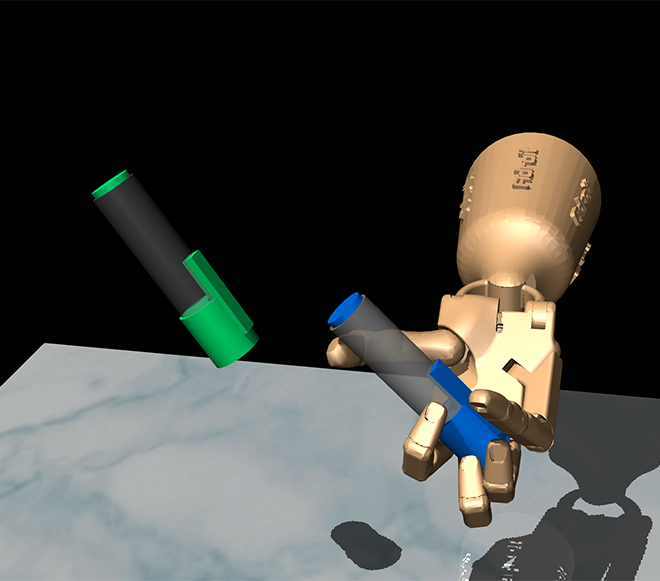
\includegraphics[height=0.6\textwidth]{awac/figures/imgs/pen.jpg}
    % \end{subfigure}
    % \begin{subfigure}[b]{0.3\textwidth}
    %     \center
    %     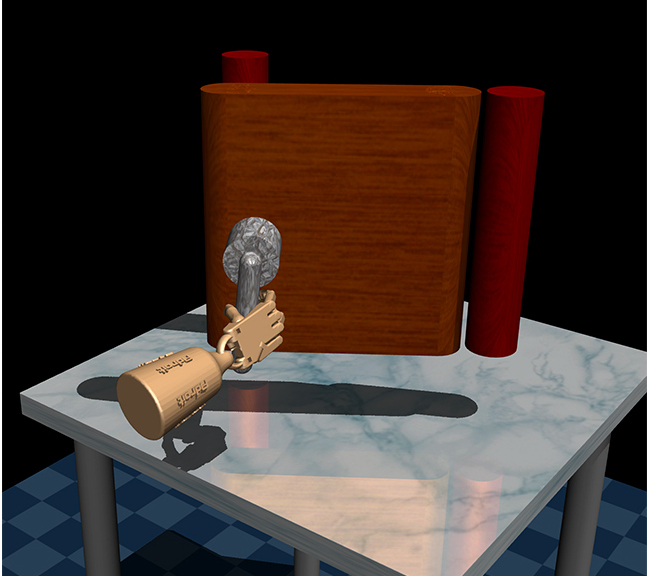
\includegraphics[height=0.6\textwidth]{awac/figures/imgs/door.jpg}
    % \end{subfigure}
    % \begin{subfigure}[b]{0.3\textwidth}
    %     \center
    %     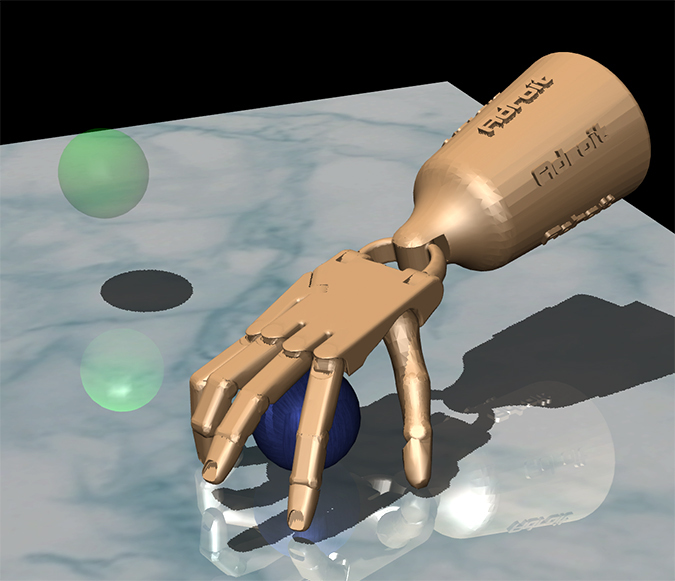
\includegraphics[height=0.6\textwidth]{awac/figures/imgs/relocate.jpg}
    % \end{subfigure}
    % \vspace{0.2cm}
    
    % \begin{subfigure}[b]{0.42\textwidth}
    %     \center
    %     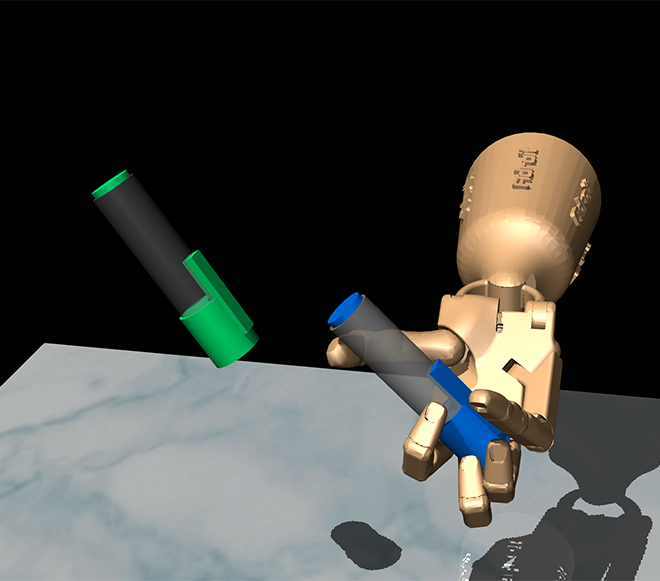
\includegraphics[height=0.26\textwidth]{awac/figures/imgs/pen.jpg}
    %     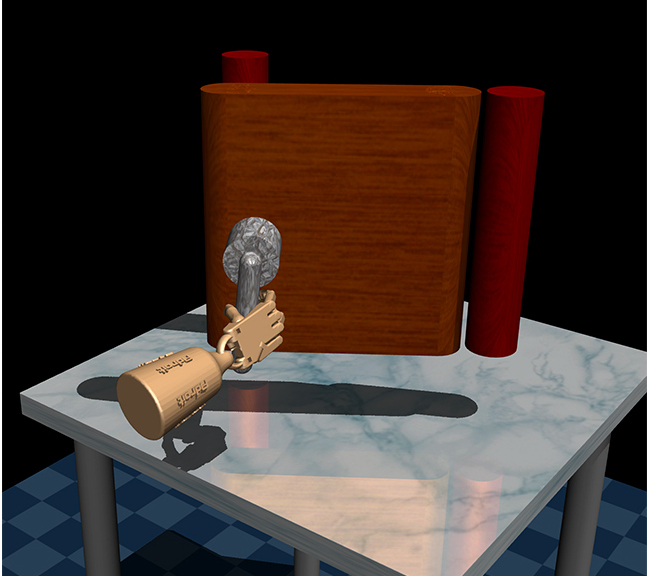
\includegraphics[height=0.26\textwidth]{awac/figures/imgs/door.jpg}
    %     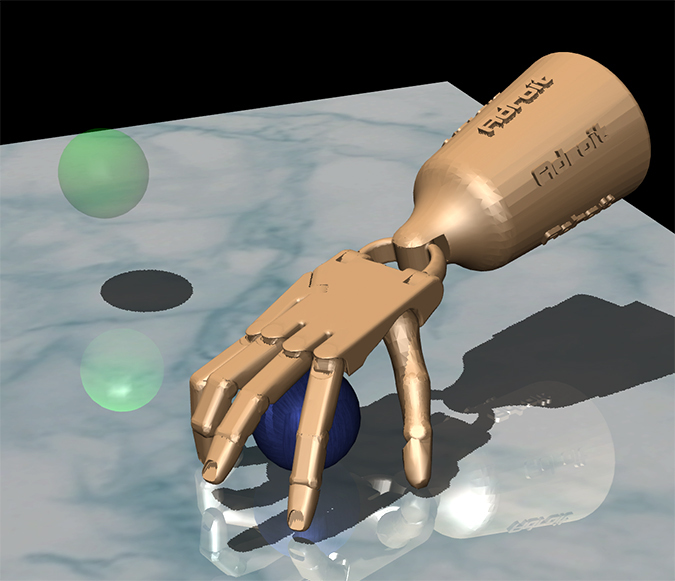
\includegraphics[height=0.26\textwidth]{awac/figures/imgs/relocate.jpg}
    % \end{subfigure}
    % \begin{subfigure}[b]{0.42\textwidth}
    %     \center
    %     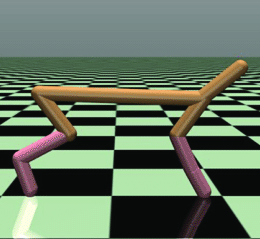
\includegraphics[height=0.26\textwidth]{awac/figures/imgs/hc.png}
    %     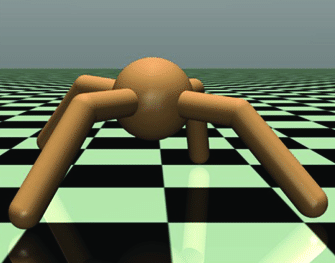
\includegraphics[height=0.26\textwidth]{awac/figures/imgs/ant.png}
    %     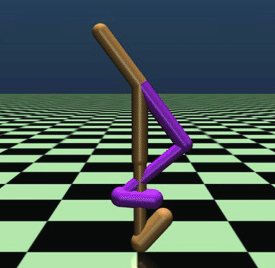
\includegraphics[height=0.26\textwidth]{awac/figures/imgs/walker.png}
    % \end{subfigure}
    % \begin{subfigure}[b]{0.14\textwidth}
    %     \center
    %     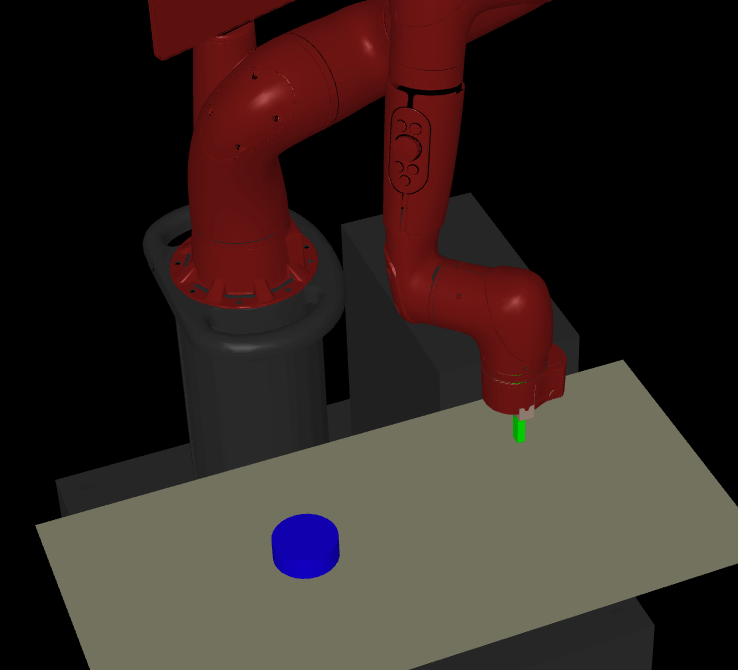
\includegraphics[height=0.78\textwidth]{awac/figures/imgs/sawyer_push.png}
    % \end{subfigure}
    % \vspace{0.2cm}
    
    \centering
    \begin{subfigure}[b]{0.02\textwidth}
        \center
        \begin{turn}{90} 
            \footnotesize
            Success Rate
        \end{turn}
        \vspace{1cm}
    \end{subfigure}
    \begin{subfigure}[b]{0.3\textwidth}
        \center
        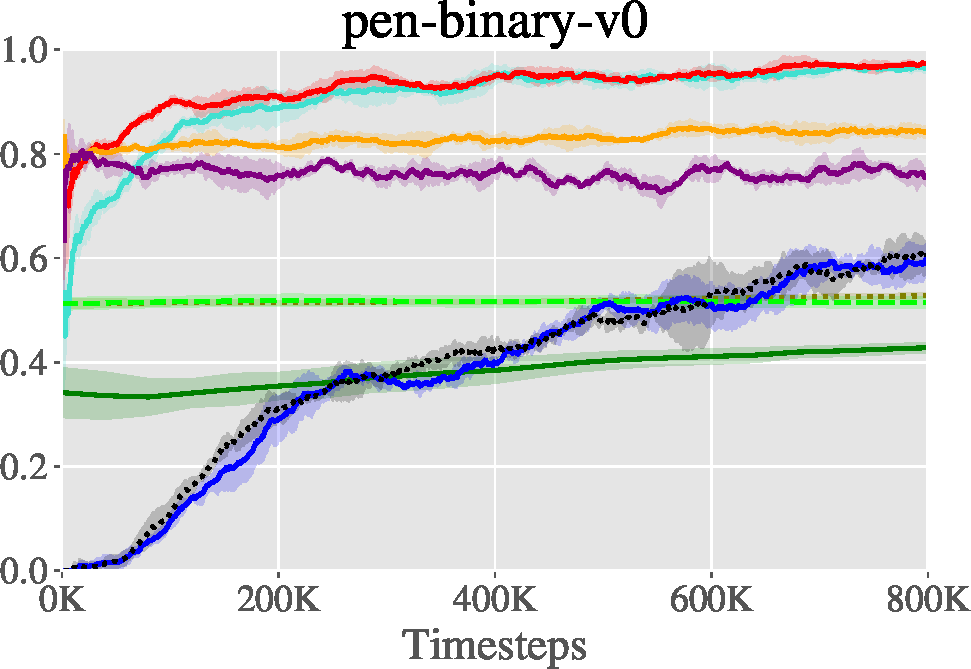
\includegraphics[width=1\textwidth]{awac/figures/hand/pen-crop.pdf}
    \end{subfigure}
    \begin{subfigure}[b]{0.3\textwidth}
        \center
        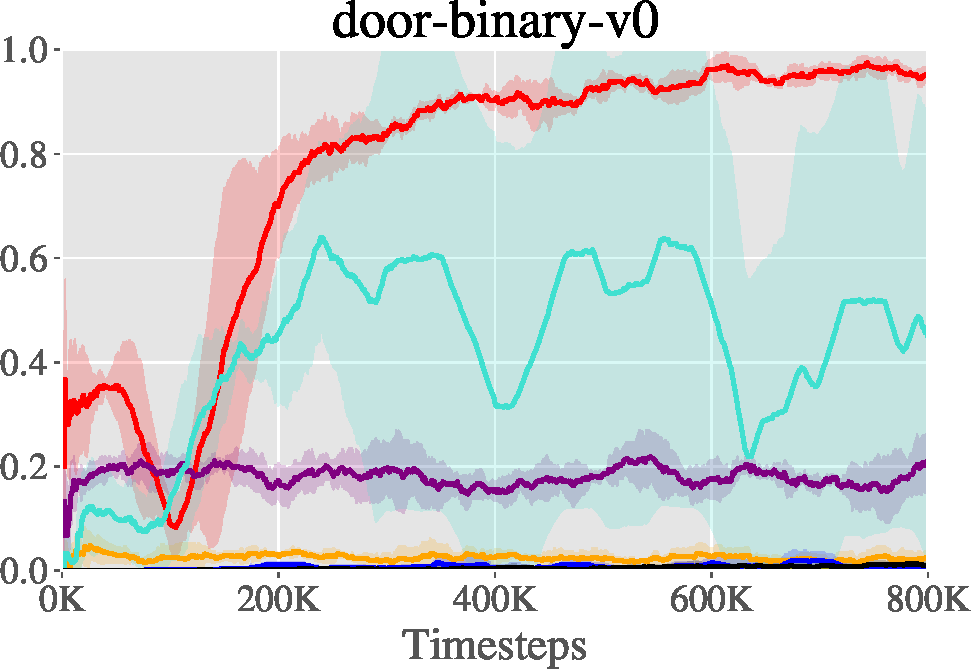
\includegraphics[width=1\textwidth]{awac/figures/hand/door-crop.pdf}
    \end{subfigure}
    \begin{subfigure}[b]{0.3\textwidth}
        \center
        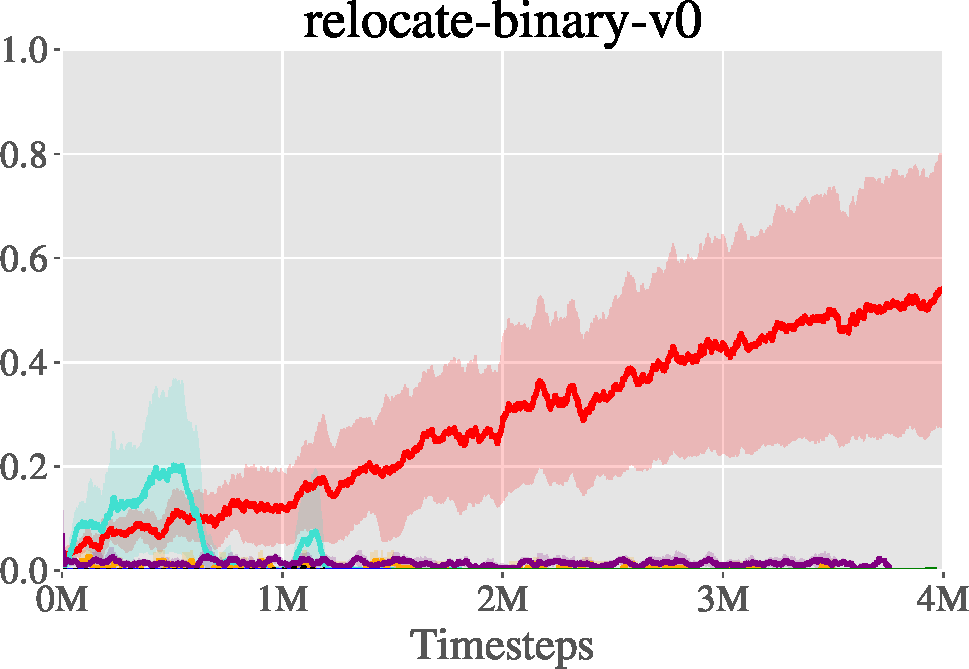
\includegraphics[width=1\textwidth]{awac/figures/hand/relocate-crop.pdf}
    \end{subfigure}
    
    \begin{subfigure}[b]{0.99\textwidth}
        \center
        % 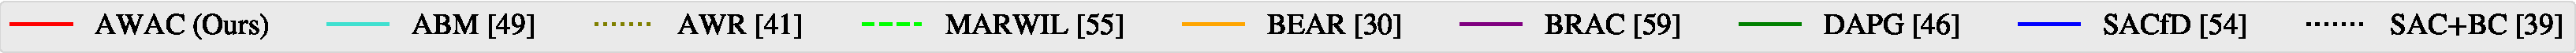
\includegraphics[width=1\textwidth]{awac/figures/mujoco/legend_ncol1-crop.pdf}
        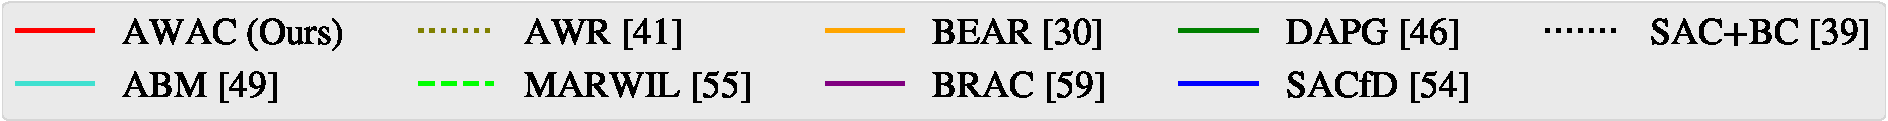
\includegraphics[width=0.6\textwidth]{awac/figures/mujoco/legend_ncol2-crop.pdf}
        % \vspace{0.2cm}
    \end{subfigure}

    \caption{
    % \footnotesize{
    Comparative evaluation on the dexterous manipulation tasks. These tasks are difficult due to their high action dimensionality and reward sparsity. We see that AWAC is able to learn these tasks with little online data collection required (100K samples $\approx$ 16 minutes of equivalent real-world interaction time). Meanwhile, most prior methods are not able to solve the harder two tasks: door opening and object relocation. 
    % ABM \cite{siegel2020abm} AWR \cite{peng2019awr} MARWIL \cite{wang2018marwil} BEAR \cite{kumar19bear} BRAC \cite{wu2019brac} DAPG \cite{rajeswaran2018dextrous} SACfD \cite{vecerik17ddpgfd} SAC+BC \cite{nair2018demonstrations}
    % }
    %\vspace{-0.5cm}
    }
    \label{fig:hand-learning-curves}
\end{figure*}
